\documentclass[tikz,border=4pt]{standalone}
\usepackage[T1]{fontenc}
\usepackage{lmodern}
\usepackage{xcolor}
\usetikzlibrary{arrows.meta,calc,positioning}

\definecolor{vbteal}{RGB}{94,170,160}
\definecolor{vbgray}{RGB}{110,110,110}

\begin{document}
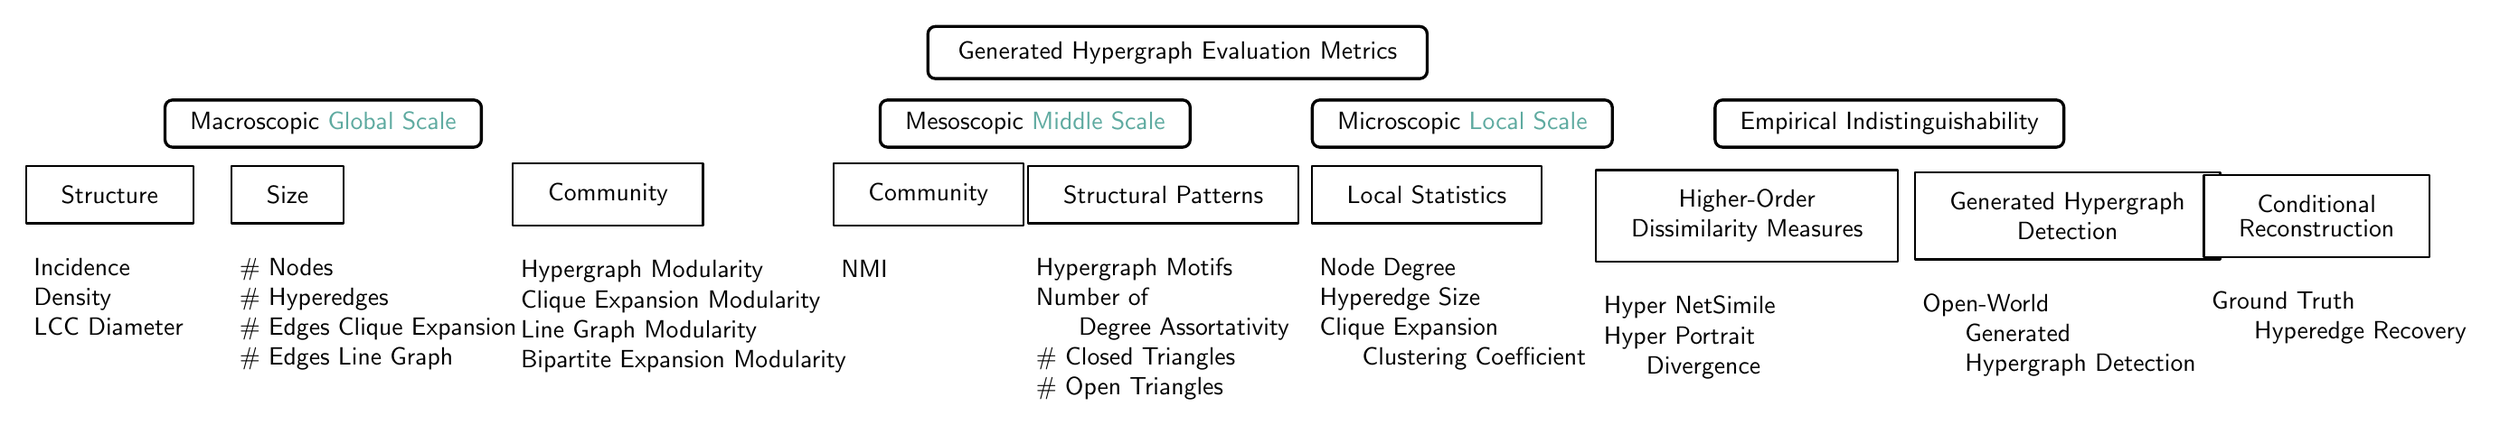
\begin{tikzpicture}[
  font=\sffamily,
  >=Stealth,
  line cap=round,
  line join=round,
  header/.style={draw=black, rounded corners=3pt, very thick, fill=white, inner xsep=12pt, inner ysep=6pt},
  cat/.style   ={draw=black, rounded corners=3pt, very thick, fill=white, inner xsep=10pt, inner ysep=5pt},
  sub/.style   ={draw=black, thick, fill=white, inner xsep=14pt, inner ysep=8pt},
  conn/.style  ={draw=vbgray, line width=2.2pt, -{Stealth[length=3.2mm,width=2.4mm]}}
]

% --- Top header --------------------------------------------------------------
\node[header] (T) at (0,0) {Generated Hypergraph Evaluation Metrics};

% --- Main category headers ---------------------------------------------------
\node[cat] (MAC) at (-12,-1) {Macroscopic \textcolor{vbteal}{Global Scale}};
\node[cat] (MES) at ( -2,-1) {Mesoscopic \textcolor{vbteal}{Middle Scale}};
\node[cat] (MIC) at (  4,-1) {Microscopic \textcolor{vbteal}{Local Scale}};
\node[cat] (EMP) at ( 10,-1) {Empirical Indistinguishability};

% --- Gray top connectors (as in the figure) ---------------------------------
% left big elbow to Macroscopic
% \draw[conn] ($(T.west)+(0,0)$) -- ++(-0.0,0) -- ++(-3,-0.5) -- ($(MAC.north)+(0,0.55)$) -- (MAC.north);

% center down then split to Mesoscopic & Microscopic
% \coordinate (C) at ($(T.south)+(0,-0.7)$);
% \draw[conn] (T.south) -- (C);
% \draw[conn] (C) -- ($(MES.north)+(0,0.55)$) -- (MES.north);
% \draw[conn] (C) -- ($(MIC.north)+(0,0.55)$) -- (MIC.north);

% right big elbow to Empirical
% \draw[conn] ($(T.north east)+(-0.2,0)$) -- ++(0,0) -- ++(0,-1.15) -- ($(EMP.north)+(0,0.55)$) -- (EMP.north);

% --- Subcategory boxes under Macroscopic ------------------------------------
\node[sub] (S1) at (-15,-2) {Structure};
\node[sub] (S2) at (-12.5,-2) {Size};
\node[sub] (S3) at (-8,-2) {Community};

% \draw[conn] (MAC.south) -- ++(0,-0.35) coordinate (mDown);
% \draw[conn] (mDown) -- (S1.north);
% \draw[conn] (mDown) -- (S2.north);
% \draw[conn] (mDown) -- (S3.north);

% Lists (Macroscopic)
\node[anchor=north west, align=left] at ($(S1.south west)+(0.0,-0.35)$) {%
Incidence\\
Density\\
LCC Diameter%
};

\node[anchor=north west, align=left] at ($(S2.south west)+(0.0,-0.35)$) {%
\# Nodes\\
\# Hyperedges\\
\# Edges Clique Expansion\\
\# Edges Line Graph%
};

\node[anchor=north west, align=left] at ($(S3.south west)+(0.0,-0.35)$) {%
Hypergraph Modularity\\
Clique Expansion Modularity\\
Line Graph Modularity\\
Bipartite Expansion Modularity%
};

% --- Subcategory boxes under Mesoscopic -------------------------------------
\node[sub] (M1) at (-3.5,-2) {Community};
\node[sub] (M2) at ( -.2,-2) {Structural Patterns};

% \draw[conn] (MES.south) -- ++(0,-0.35) coordinate (mesDown);
% \draw[conn] (mesDown) -- (M1.north);
% \draw[conn] (mesDown) -- (M2.north);

\node[anchor=north west, align=left] at ($(M1.south west)+(0.0,-0.35)$) {%
NMI%
};

\node[anchor=north west, align=left] at ($(M2.south west)+(0.0,-0.35)$) {%
Hypergraph Motifs\\
Number of\\
\hspace*{1.7em}Degree Assortativity\\
\# Closed Triangles\\
\# Open Triangles%
};

% --- Subcategory boxes under Microscopic ------------------------------------
\node[sub] (L1) at ( 3.5,-2) {Local Statistics};

% \draw[conn] (MIC.south) -- ++(0,-0.35) -- (L1.north);

\node[anchor=north west, align=left] at ($(L1.south west)+(0.0,-0.35)$) {%
Node Degree\\
Hyperedge Size\\
Clique Expansion\\
\hspace*{1.7em}Clustering Coefficient%
};

% --- Subcategory boxes under Empirical Indistinguishability -----------------
\node[sub] (E1) at ( 8,-2.3) {\shortstack{Higher-Order\\Dissimilarity Measures}};
\node[sub] (E2) at (12.5,-2.3) {\shortstack{Generated Hypergraph\\Detection}};
\node[sub] (E3) at (16,-2.3) {\shortstack{Conditional \\Reconstruction}};

% bracket-like connector under EMP, then three down arrows
% \coordinate (eL) at ($(E1.north)+(0,0.45)$);
% \coordinate (eR) at ($(E3.north)+(0,0.45)$);
% \draw[conn] (EMP.south) -- ++(0,-0.22) coordinate (empStem);
% \draw[conn] (empStem) -- ++(-3.25,0) coordinate (empLeft);
% \draw[conn] (empStem) -- ++( 3.25,0) coordinate (empRight);
% \draw[conn] (empLeft) -- (eL);
% \draw[conn] (empRight) -- (eR);
% \draw[conn] ($(E2.north)+(0,0.45)$) -- (E2.north);
% \draw[conn] (eL) -- (E1.north);
% \draw[conn] (eR) -- (E3.north);

% Lists (Empirical)
\node[anchor=north west, align=left] at ($(E1.south west)+(0.0,-0.35)$) {%
Hyper NetSimile\\
Hyper Portrait\\
\hspace*{1.7em}Divergence%
};

\node[anchor=north west, align=left] at ($(E2.south west)+(0.0,-0.35)$) {%
Open-World\\
\hspace*{1.7em}Generated\\
\hspace*{1.7em}Hypergraph Detection%
};

\node[anchor=north west, align=left] at ($(E3.south west)+(0.0,-0.35)$) {%
Ground Truth\\
\hspace*{1.7em}Hyperedge Recovery%
};

\end{tikzpicture}
\end{document}